\label{sec:overview}

\subsection{Background of False Sharing}
\label{sec:background}

In the multicore era, multithreading is the basic way to utilize underlying hardware cores by running different threads on different cores. When a thread modifies data of a cache line, the underlying cache coherence protocol (inside hardware) silently invalidates the duplicates of this cache line on other cores. This is to guarantee correct executions for true sharing instances like that shown in Figure~\ref{fig:tsinfs}. However, for false sharing case (e.g. Figure~\ref{fig:fsinfs}), these invalidations are totally unnecessary when different tasks are actually accessing different words of the same line. Cache invalidations may force other cores to wait for reloading of data unnecessarily, wasting CPU time and precious memory bandwidth. A big amount of unnecessary cache invalidations can hugely affect the performance of software. %Thus, it is urgent to develop some tools and systems to tackle with this problem. 

\begin{figure}[htbp]
\centering
\subfigure[False sharing]{%
   \label{fig:fsinfs}
   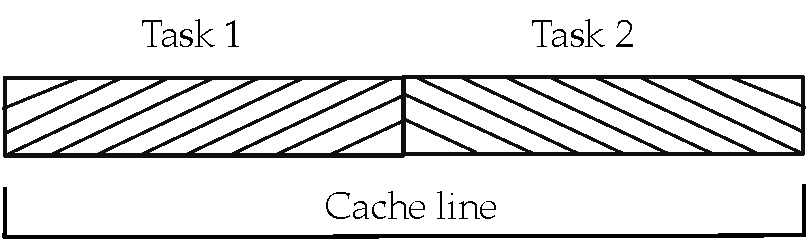
\includegraphics[width=2.4in]{figure/falsesharing}
}%
\hspace{30pt}
\subfigure[True sharing]{%
   \label{fig:tsinfs}
   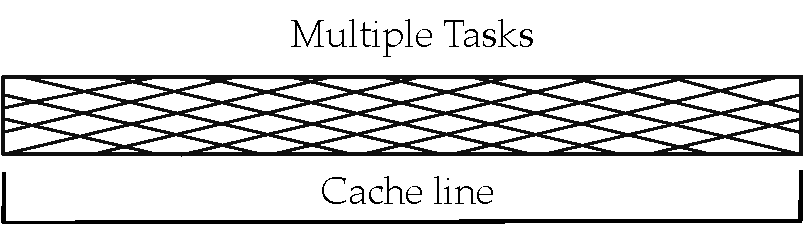
\includegraphics[width=2.4in]{figure/truesharing}
}%
\caption{False sharing (a) vs. true sharing (b). For false sharing, different tasks access different parts of the same cache line simultaneously. For true sharing, multiple tasks access the same part of a cache line.\label{fig:falsesharing}}
\end{figure}

False sharing can be categorized into inter-object and intra-object false sharing. When two different objects in the same cache line are accessed by different threads simultaneously, that is inter-object false sharing. Otherwise, it is intra-object false sharing. Generally, false sharing is avoidable, while true sharing is not. 

Common programming practice can easily introduce false sharing. For example, different threads may access different words of the same global array, as the example in Figure~\ref{fig:penaltycode}. There are several ways to fix false sharing problems by preventing multiple threads from accessing the same cache line simultaneously. {\tt First},  we can pad useless words into a corresponding structure or class. {\tt Second}, we can assign the value of falsely-shared variable to a thread-local variable so that different threads may update their local variables, and commit those changes back to the shared variable in the end. {\tt Third}, Sheriff isolates the execution of different threads by turning threads into processes~\cite{sheriff}. However, Sheriff only works for multithreaded programs that are using the standard \pthreads{} library, without ad hoc synchronizations~\cite{Xiong:2010:AHS:1924943.1924955} and communication across the stack. For the first two approaches, programmers should have precise information about falsely-shared objects in order to fix them. \cheetah{} aims to provide precise information as much as possible, such as where are those objects, what is access pattern, and how much performance improvement after fixes. 

\subsection{Basic Idea of Detection}
\label{sec:basicidea}
% What is the basic idea? Why those ones uses performance counters can not reveal false sharing problems? 
\cheetah{} aims to report both read-write and write-write false sharing that may have performance impact, where a large number of cache invalidations occur on those cache lines. However, it is not easy to know whether a cache line is invalidated or not, without the complete information of cache hierarchy and different threads' running situation. 

\cheetah{} eliminates the need for knowing cache hierarchy and running information of threads. \cheetah{} computes the number of cache invalidations according to a basic rule: {\it \bf if a task writes a cache line after other tasks have accessed this cache line, this write operation causes a cache invalidation}. To make it true, \cheetah{} further makes the following \textbf{two basic assumptions}, which is similar to previous work~\cite{qinzhao, Predator}.

\begin{itemize} 
\item {\bf Assumption 1:} Each task runs on a separate core with its own cache. 

\item {\bf Assumption 2: } The sizes of caches are infinite. 
 
\end{itemize}

Assumption 1 is a reasonable assumption since different tasks can run on a separate core, even if they may not in a given execution. Given this assumption, we do not need to know the actual running condition of different tasks. After we assume that different cores have their own cache (at least L1 cache), we can avoid the complexity of knowing actual cache hierarchy. 

Assumption 2 further assumes that the sizes of caches are infinite. Thus, we do not need to track cache evictions. If there is a memory access within a cache line, this cache always holds the data until an access of other tasks (running on other cores) invalidates it. Because a memory access of a task will load this cache line on its own cache (assumption 1), then a write from a different task can invalidate this cache line. Thus, the basic rule described above is always valid given these two assumptions.  

 
% This idea is similar to Predator. But Predator is a compiler-based approach, which needs to change the source code of applications. Also, it introduces much performance overhead that can block its use in deployment environment. 

% To reduce the performance overhead, 
% Basic idea, by examing the memory access pattern

\subsubsection{Sampling Memory Accesses Using Performance Counters}
\label{sec:perfcounter}

According to the basic rule described in Section~\ref{sec:basicidea}, we should track memory accesses in order to compute the number of cache invalidations on each cache line. 


The previous work \Predator{} leverages on compiler instrumentation to insert function calls before every memory access that is going to handled by \Predator{}'s runtime system~\cite{Predator}. However, this approach introduces more than $5\times$ performance overhead by tracking every memory access. More than that, \Predator{} has to re-compile applications, which needs the availability of source code. \Predator{} is not desirable for legacy applications or real deployment that is sensitive to performance. 

\cheetah{} aims to significantly reduce the performance overhead of tracking memory accesses by leveraging hardware performance counters that are available on most modern hardware. Hardware performance counters can provide sampling based information about how the hardware is being exercised by a program, which have been utilized widely for different purposes~\cite{Mucci99papi}. Performance counters were also utilized by previous work to identify false sharing problems. But existing work suffered from different problems, which has been discussed in Section~\ref{sec:relatedwork}. All of them can not differentiate false sharing with true sharing. 
 
Using performance counters does not need to instrument source code explicitly, thus providing a non-intrusive way to monitor memory references. 
Different with previous tools ~\cite{mldetect, openmp, detect:ptu}, \cheetah{} only needs sample memory read and write accesses and relies on the basic rule that are discussed in Section~\ref{sec:basicidea} to track the number of cache invalidations on every cache line. \Cheetah{} relies on AMD's IBS registers to track specific memory accesses. The details of tracking cache invalidations is discussed in Section~\ref{sec:computeinvalidations}. 

\subsubsection{Computing Cache Invalidations}
\label{sec:computeinvalidations}

\Cheetah{} targets to report false sharing that can have performance impact on applications. Since a big number of cache invalidations are the culprit of performance problems, \Cheetah{}  computes the number of cache invalidations on each cache line and reports those ones with a significant number of cache invalidations.  

Qin Zhao et. al. propose to compute the number of cache invalidations based on the ownership of cache lines: when a thread updates an object that it does not own, it will cause cache invalidations and set the owner to the current thread~\cite{qinzhao}. However, this approach cannot be easily to scalable to more than 32 threads because of excessive memory consumption, where every word of memory will at least occupy a 32-bits word for tracking ownership, and performance overhead of maintaining ownership of cache lines. Instead, \Cheetah{} utilizes a similar mechanism as \Predator{}~\cite{Predator}. 

\cheetah{} maintains a two-entries-table ($T$) for each cache line ($L$), where each entry tracks accesses from a thread. It also keeps a counter for every cache line that indicates the number of cache invalidation on this cache line.  
According to the basic rule that are described in Section~\ref{sec:basicidea}, only a write access can cause cache invalidation. When there is a cache invalidation, the current write access will flush the table and will be added into its corresponding table ($T$). Thus, a table will always have an entry except in the beginning. More specifically, \cheetah{} checks possible cache invalidations as follows.
 
\begin{itemize}
\item
  For each read access $R$,
  \begin{itemize}
    \item
      If $T$ is full, there is no need to record this read access.
    \item
      If $T$ is not full and the existing entry has a different task ID, 
      then \cheetah{} records this read access by adding a new entry to the table.
  \end{itemize}
\item
  For each write access $W$,  
  \begin{itemize}
    \item
      If $T$ is full, then $W$ causes a cache invalidation since at least one of two existing entries are issued by another task (on another core).
    \item
      If $T$ is not full (and not empty),
      \cheetah{} checks whether $W$ and the existing entry have the same task ID. If
      so, $W$ will not cause a cache invalidation. Otherwise, there is a cache invalidation caused by this $W$.
  \end{itemize}
\end{itemize}

      
After the computation, 
%\cheetah{} ranks the severity of performance degradation of any detected false sharing problems according to the number of cache invalidations. 
\cheetah{} only reports those false sharing problems that can have a significant impact on the performance by predicting the upper bound of performance improvement, according to the idea that are discussed in Section~\ref{sec:predictimprovement}.  It will rank the severity of performance degradation of any detected false sharing problems based on the predicted performance improvement after fixes.

\subsection{Basic Idea of Predicting Performance Improvement}
\label{sec:predictimprovement}

\paragraph{Current problem:} Existing tools cannot predict whether fixing a false sharing problem can improve the performance or not~\cite{sheriff, Predator, openmp}. They might report some insignificant false sharing problems even when the number of cache invalidations on a cache line is over a pre-defined threshold. For example, all of these tools report an false sharing problem at reverse\_index application of the Phoenix benchmark suite but there is no significant performance improvement after fixing it. Unnecessary false sharing instances are not false positives, but reporting them increases burden for programmers and will not bring the performance improvement after fixes. Different with all existing tools, \Cheetah{} only reports false sharing problems that can have performance impact based on its prediction of performance improvement.  

{\bf \Cheetah{} is the first tool that can predict performance improvement after fixes}, which utilizes the latency information (e.g. cycles) of every memory access that can be provided by either Intel's PEBS registers or AMD's IBS registers. \Cheetah{} considers the sum of cycles to be the running time. \Cheetah{} further use the sampling result to represent the whole execution, which is reasonable given that sampling is evenly distributed among the whole execution. 
%Note that it is difficult or even impossible to precisely predict the performance improvement after fixes. For example, sharing of cache lines can be different or fixing a false sharing may introduce performance variance. 

\Cheetah{} aims to predict a upper bound of performance improvement percentage, but not an absolute value of time saving. We believe that this is more valuable since programmers can only focus on false sharing problems that fixing them can bring the performance improvement, e.g., with more than 2\% performance improvement.   

According to our understanding, the actual runtime (denoted as $Runtime_{real}$) is the sum of the actual runtime spending on the current object ($Runtime_{obj\_real}$) and the actual runtime spending on other objects or variables ($Runtime_{others\_real}$). Because of this, we will have the EQ.(\ref{eq:actual}). 

\begin{equation}
\label{eq:actual}
Runtime_{real}=Runtime_{obj\_real} + Runtime_{others\_real}
\end{equation} 

{\it We further assume that fixing an false sharing problem will not introduce performance impact on other variables or objects}. If we fix false sharing of an object, the predicted runtime after fixing ($Runtime_{pred}$) is the sum of the predicted time spending on the current object ($Runtime_{obj\_pred}$) and the actual runtime spending on other objects or variables ($Runtime_{others\_real}$), we will have the EQ.(\ref{eq:pred}). 

\begin{equation}
\label{eq:pred}
Runtime_{pred}=Runtime_{obj\_pred}+Runtime_{others\_real}
\end{equation} 

Based on these two equations, we can easily compute the performance improvement (denoted as $Perf_{improve}$) after fixing a specific false sharing, shown as EQ.(\ref{eq:improvement}). 
\begin{equation}
\label{eq:improvement}
Perf_{improve}=(Runtime_{actual} - Runtime_{pred})/Runtime_{actual}
\end{equation} 

According to EQ.(\ref{eq:improvement}), predicting performance improvement turns into the computation of $Runtime_{pred}$. $Runtime_{actual}$ can be easily computed through the sampling result if we have the latency information of every memory access and we are using the sampling result to represent the whole execution.  

{\bf The basic idea of predicting the running time spending on a falsely-shared object is to replace the actual access latency of every memory access with the average access latency of an access without false sharing}. In actual fixes,   padding unnecessary words into structures or classes (as described in Section~\ref{sec:background}) can reduce the memory efficiency and may even degrade the performance of an application~\cite{qinzhao}. Thus, our prediction actually provides an upper bound of performance improvement that can be achieved by fixes. More implementation details about how to compute the $Runtime_{pred}$ and $Runtime_{actual}$ are further discussed in Section~\ref{sec:predictimprove}. We also evaluate the precision of our prediction in Section~\ref{sec:evalperfpred}.


